\documentclass[1p]{elsarticle_modified}
%\bibliographystyle{elsarticle-num}

%\usepackage[colorlinks]{hyperref}
%\usepackage{abbrmath_seonhwa} %\Abb, \Ascr, \Acal ,\Abf, \Afrak
\usepackage{amsfonts}
\usepackage{amssymb}
\usepackage{amsmath}
\usepackage{amsthm}
\usepackage{scalefnt}
\usepackage{amsbsy}
\usepackage{kotex}
\usepackage{caption}
\usepackage{subfig}
\usepackage{color}
\usepackage{graphicx}
\usepackage{xcolor} %% white, black, red, green, blue, cyan, magenta, yellow
\usepackage{float}
\usepackage{setspace}
\usepackage{hyperref}

\usepackage{tikz}
\usetikzlibrary{arrows}

\usepackage{multirow}
\usepackage{array} % fixed length table
\usepackage{hhline}

%%%%%%%%%%%%%%%%%%%%%
\makeatletter
\renewcommand*\env@matrix[1][\arraystretch]{%
	\edef\arraystretch{#1}%
	\hskip -\arraycolsep
	\let\@ifnextchar\new@ifnextchar
	\array{*\c@MaxMatrixCols c}}
\makeatother %https://tex.stackexchange.com/questions/14071/how-can-i-increase-the-line-spacing-in-a-matrix
%%%%%%%%%%%%%%%

\usepackage[normalem]{ulem}

\newcommand{\msout}[1]{\ifmmode\text{\sout{\ensuremath{#1}}}\else\sout{#1}\fi}
%SOURCE: \msout is \stkout macro in https://tex.stackexchange.com/questions/20609/strikeout-in-math-mode

\newcommand{\cancel}[1]{
	\ifmmode
	{\color{red}\msout{#1}}
	\else
	{\color{red}\sout{#1}}
	\fi
}

\newcommand{\add}[1]{
	{\color{blue}\uwave{#1}}
}

\newcommand{\replace}[2]{
	\ifmmode
	{\color{red}\msout{#1}}{\color{blue}\uwave{#2}}
	\else
	{\color{red}\sout{#1}}{\color{blue}\uwave{#2}}
	\fi
}

\newcommand{\Sol}{\mathcal{S}} %segment
\newcommand{\D}{D} %diagram
\newcommand{\A}{\mathcal{A}} %arc


%%%%%%%%%%%%%%%%%%%%%%%%%%%%%5 test

\def\sl{\operatorname{\textup{SL}}(2,\Cbb)}
\def\psl{\operatorname{\textup{PSL}}(2,\Cbb)}
\def\quan{\mkern 1mu \triangleright \mkern 1mu}

\theoremstyle{definition}
\newtheorem{thm}{Theorem}[section]
\newtheorem{prop}[thm]{Proposition}
\newtheorem{lem}[thm]{Lemma}
\newtheorem{ques}[thm]{Question}
\newtheorem{cor}[thm]{Corollary}
\newtheorem{defn}[thm]{Definition}
\newtheorem{exam}[thm]{Example}
\newtheorem{rmk}[thm]{Remark}
\newtheorem{alg}[thm]{Algorithm}

\newcommand{\I}{\sqrt{-1}}
\begin{document}

%\begin{frontmatter}
%
%\title{Boundary parabolic representations of knots up to 8 crossings}
%
%%% Group authors per affiliation:
%\author{Yunhi Cho} 
%\address{Department of Mathematics, University of Seoul, Seoul, Korea}
%\ead{yhcho@uos.ac.kr}
%
%
%\author{Seonhwa Kim} %\fnref{s_kim}}
%\address{Center for Geometry and Physics, Institute for Basic Science, Pohang, 37673, Korea}
%\ead{ryeona17@ibs.re.kr}
%
%\author{Hyuk Kim}
%\address{Department of Mathematical Sciences, Seoul National University, Seoul 08826, Korea}
%\ead{hyukkim@snu.ac.kr}
%
%\author{Seokbeom Yoon}
%\address{Department of Mathematical Sciences, Seoul National University, Seoul, 08826,  Korea}
%\ead{sbyoon15@snu.ac.kr}
%
%\begin{abstract}
%We find all boundary parabolic representation of knots up to 8 crossings.
%
%\end{abstract}
%\begin{keyword}
%    \MSC[2010] 57M25 
%\end{keyword}
%
%\end{frontmatter}

%\linenumbers
%\tableofcontents
%
\newcommand\colored[1]{\textcolor{white}{\rule[-0.35ex]{0.8em}{1.4ex}}\kern-0.8em\color{red} #1}%
%\newcommand\colored[1]{\textcolor{white}{ #1}\kern-2.17ex	\textcolor{white}{ #1}\kern-1.81ex	\textcolor{white}{ #1}\kern-2.15ex\color{red}#1	}

{\Large $\underline{12n_{0172}~(K12n_{0172})}$}

\setlength{\tabcolsep}{10pt}
\renewcommand{\arraystretch}{1.6}
\vspace{1cm}\begin{tabular}{m{100pt}>{\centering\arraybackslash}m{274pt}}
\multirow{5}{120pt}{
	\centering
	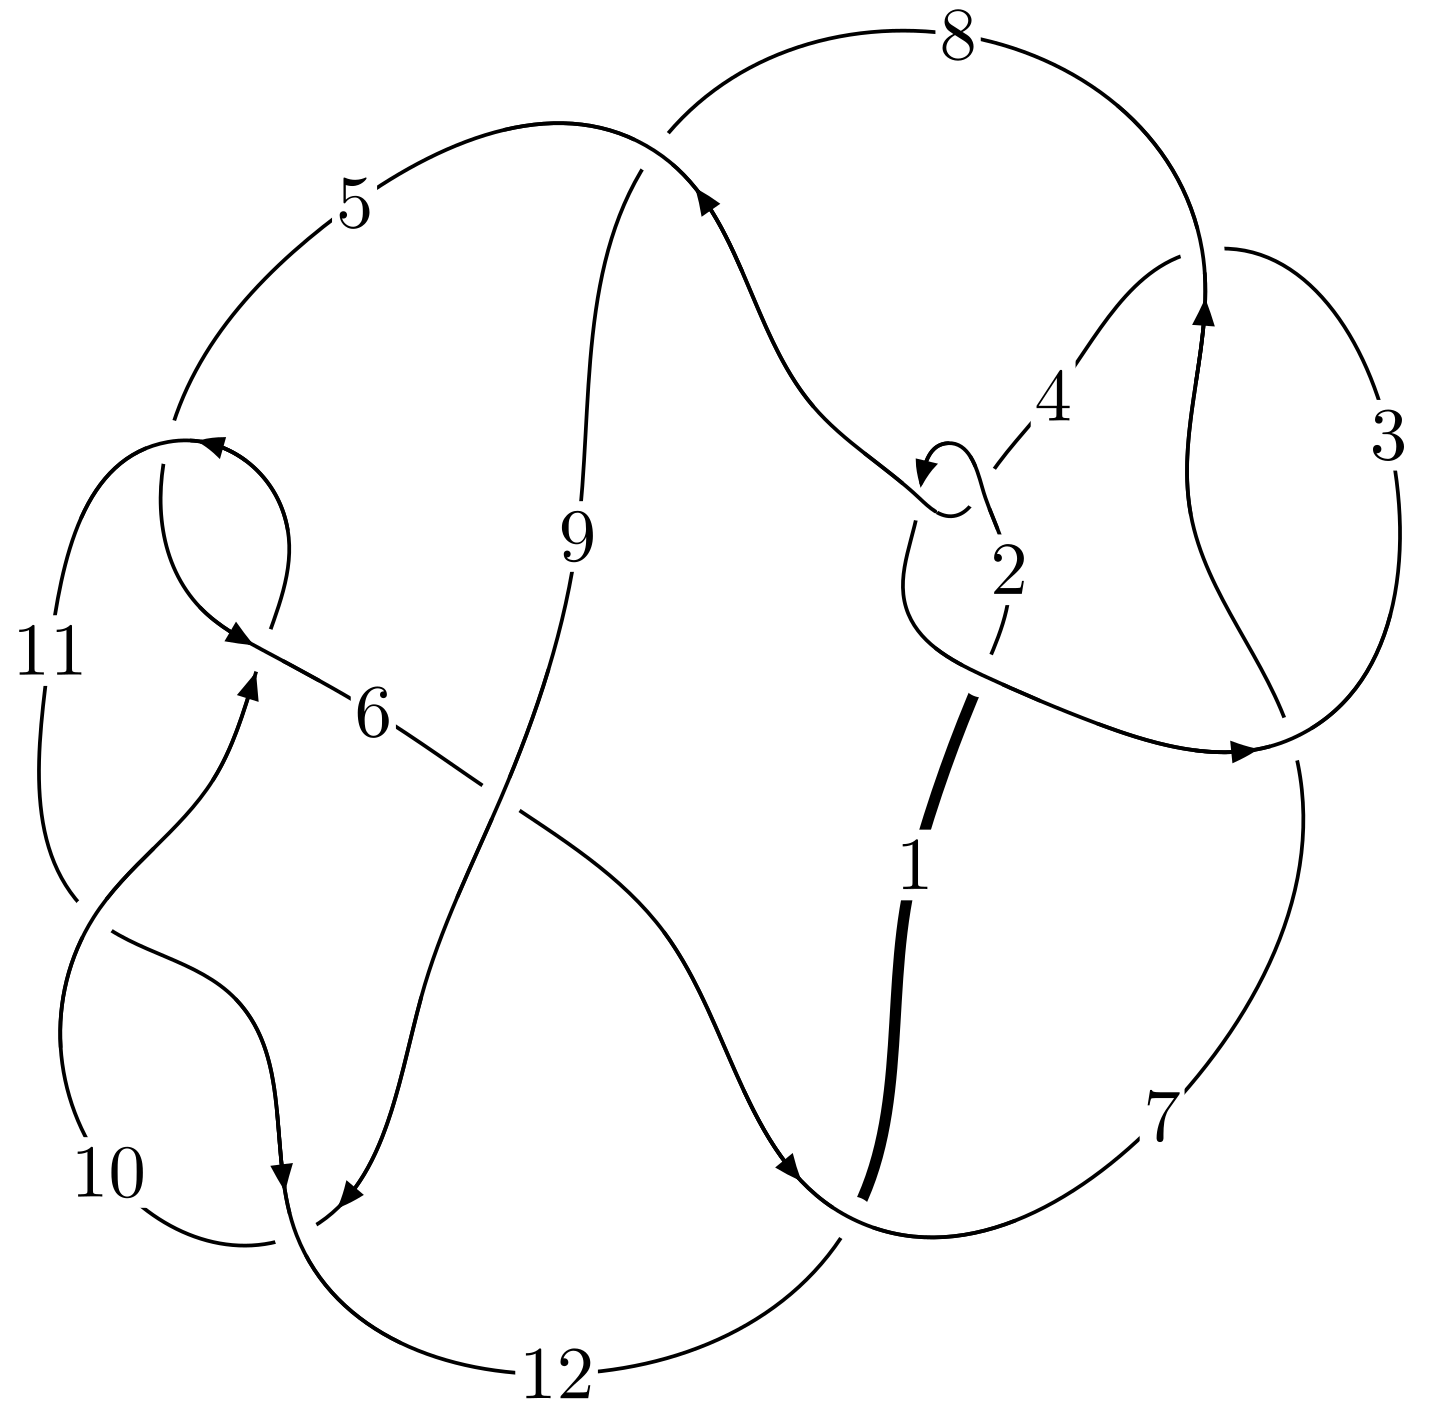
\includegraphics[width=112pt]{../../../GIT/diagram.site/Diagrams/png/2261_12n_0172.png}\\
\ \ \ A knot diagram\footnotemark}&
\allowdisplaybreaks
\textbf{Linearized knot diagam} \\
\cline{2-2}
 &
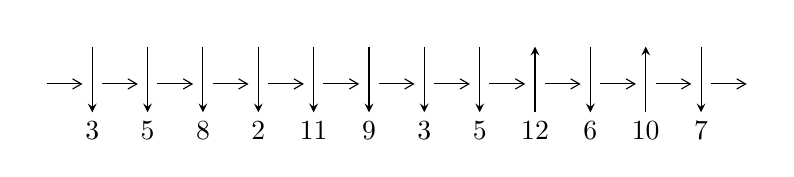
\begin{tikzpicture}[x=20pt, y=17pt]
	% nodes
	\node (C0) at (0, 0) {};
	\node (C1) at (1, 0) {};
	\node (C1U) at (1, +1) {};
	\node (C1D) at (1, -1) {3};

	\node (C2) at (2, 0) {};
	\node (C2U) at (2, +1) {};
	\node (C2D) at (2, -1) {5};

	\node (C3) at (3, 0) {};
	\node (C3U) at (3, +1) {};
	\node (C3D) at (3, -1) {8};

	\node (C4) at (4, 0) {};
	\node (C4U) at (4, +1) {};
	\node (C4D) at (4, -1) {2};

	\node (C5) at (5, 0) {};
	\node (C5U) at (5, +1) {};
	\node (C5D) at (5, -1) {11};

	\node (C6) at (6, 0) {};
	\node (C6U) at (6, +1) {};
	\node (C6D) at (6, -1) {9};

	\node (C7) at (7, 0) {};
	\node (C7U) at (7, +1) {};
	\node (C7D) at (7, -1) {3};

	\node (C8) at (8, 0) {};
	\node (C8U) at (8, +1) {};
	\node (C8D) at (8, -1) {5};

	\node (C9) at (9, 0) {};
	\node (C9U) at (9, +1) {};
	\node (C9D) at (9, -1) {12};

	\node (C10) at (10, 0) {};
	\node (C10U) at (10, +1) {};
	\node (C10D) at (10, -1) {6};

	\node (C11) at (11, 0) {};
	\node (C11U) at (11, +1) {};
	\node (C11D) at (11, -1) {10};

	\node (C12) at (12, 0) {};
	\node (C12U) at (12, +1) {};
	\node (C12D) at (12, -1) {7};
	\node (C13) at (13, 0) {};

	% arrows
	\draw[->,>={angle 60}]
	(C0) edge (C1) (C1) edge (C2) (C2) edge (C3) (C3) edge (C4) (C4) edge (C5) (C5) edge (C6) (C6) edge (C7) (C7) edge (C8) (C8) edge (C9) (C9) edge (C10) (C10) edge (C11) (C11) edge (C12) (C12) edge (C13) ;	\draw[->,>=stealth]
	(C1U) edge (C1D) (C2U) edge (C2D) (C3U) edge (C3D) (C4U) edge (C4D) (C5U) edge (C5D) (C6U) edge (C6D) (C7U) edge (C7D) (C8U) edge (C8D) (C9D) edge (C9U) (C10U) edge (C10D) (C11D) edge (C11U) (C12U) edge (C12D) ;
	\end{tikzpicture} \\
\hhline{~~} \\& 
\textbf{Solving Sequence} \\ \cline{2-2} 
 &
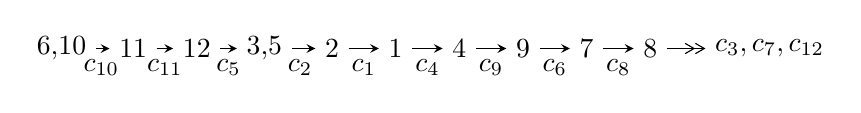
\begin{tikzpicture}[x=23pt, y=7pt]
	% node
	\node (A0) at (-1/8, 0) {6,10};
	\node (A1) at (1, 0) {11};
	\node (A2) at (2, 0) {12};
	\node (A3) at (49/16, 0) {3,5};
	\node (A4) at (33/8, 0) {2};
	\node (A5) at (41/8, 0) {1};
	\node (A6) at (49/8, 0) {4};
	\node (A7) at (57/8, 0) {9};
	\node (A8) at (65/8, 0) {7};
	\node (A9) at (73/8, 0) {8};
	\node (C1) at (1/2, -1) {$c_{10}$};
	\node (C2) at (3/2, -1) {$c_{11}$};
	\node (C3) at (5/2, -1) {$c_{5}$};
	\node (C4) at (29/8, -1) {$c_{2}$};
	\node (C5) at (37/8, -1) {$c_{1}$};
	\node (C6) at (45/8, -1) {$c_{4}$};
	\node (C7) at (53/8, -1) {$c_{9}$};
	\node (C8) at (61/8, -1) {$c_{6}$};
	\node (C9) at (69/8, -1) {$c_{8}$};
	\node (A10) at (11, 0) {$c_{3},c_{7},c_{12}$};

	% edge
	\draw[->,>=stealth]	
	(A0) edge (A1) (A1) edge (A2) (A2) edge (A3) (A3) edge (A4) (A4) edge (A5) (A5) edge (A6) (A6) edge (A7) (A7) edge (A8) (A8) edge (A9) ;
	\draw[->>,>={angle 60}]	
	(A9) edge (A10);
\end{tikzpicture} \\ 

\end{tabular} \\

\footnotetext{
The image of knot diagram is generated by the software ``\textbf{Draw programme}" developed by Andrew Bartholomew(\url{http://www.layer8.co.uk/maths/draw/index.htm\#Running-draw}), where we modified some parts for our purpose(\url{https://github.com/CATsTAILs/LinksPainter}).
}\phantom \\ \newline 
\centering \textbf{Ideals for irreducible components\footnotemark of $X_{\text{par}}$} 
 
\begin{align*}
I^u_{1}&=\langle 
- u^{19}-2 u^{18}+\cdots+b+1,\;- u^{19}- u^{18}+\cdots+a-1,\;u^{20}+2 u^{19}+\cdots-3 u-1\rangle \\
I^u_{2}&=\langle 
u^7+u^5+2 u^3+u^2+b+u,\;u^6+u^4+2 u^2+a+u+1,\;u^9- u^8+2 u^7- u^6+3 u^5- u^4+2 u^3+u+1\rangle \\
\\
\end{align*}
\raggedright * 2 irreducible components of $\dim_{\mathbb{C}}=0$, with total 29 representations.\\
\footnotetext{All coefficients of polynomials are rational numbers. But the coefficients are sometimes approximated in decimal forms when there is not enough margin.}
\newpage
\renewcommand{\arraystretch}{1}
\centering \section*{I. $I^u_{1}= \langle - u^{19}-2 u^{18}+\cdots+b+1,\;- u^{19}- u^{18}+\cdots+a-1,\;u^{20}+2 u^{19}+\cdots-3 u-1 \rangle$}
\flushleft \textbf{(i) Arc colorings}\\
\begin{tabular}{m{7pt} m{180pt} m{7pt} m{180pt} }
\flushright $a_{6}=$&$\begin{pmatrix}0\\u\end{pmatrix}$ \\
\flushright $a_{10}=$&$\begin{pmatrix}1\\0\end{pmatrix}$ \\
\flushright $a_{11}=$&$\begin{pmatrix}1\\u^2\end{pmatrix}$ \\
\flushright $a_{12}=$&$\begin{pmatrix}u^2+1\\u^2\end{pmatrix}$ \\
\flushright $a_{3}=$&$\begin{pmatrix}u^{19}+u^{18}+\cdots+u^2+1\\u^{19}+2 u^{18}+\cdots-4 u-1\end{pmatrix}$ \\
\flushright $a_{5}=$&$\begin{pmatrix}u\\u^3+u\end{pmatrix}$ \\
\flushright $a_{2}=$&$\begin{pmatrix}2 u^{19}+2 u^{18}+\cdots-4 u^3+1\\2 u^{19}+4 u^{18}+\cdots-6 u-2\end{pmatrix}$ \\
\flushright $a_{1}=$&$\begin{pmatrix}- u^{16}-3 u^{14}-7 u^{12}-10 u^{10}-11 u^8-8 u^6-4 u^4+1\\- u^{16}-2 u^{14}-4 u^{12}-4 u^{10}-2 u^8+2 u^4+2 u^2\end{pmatrix}$ \\
\flushright $a_{4}=$&$\begin{pmatrix}-3 u^{19}-3 u^{18}+\cdots+u^2+2 u\\-3 u^{19}-6 u^{18}+\cdots+9 u+3\end{pmatrix}$ \\
\flushright $a_{9}=$&$\begin{pmatrix}u^4+u^2+1\\u^4\end{pmatrix}$ \\
\flushright $a_{7}=$&$\begin{pmatrix}- u^9-2 u^7-3 u^5-2 u^3- u\\- u^9- u^7- u^5+u\end{pmatrix}$ \\
\flushright $a_{8}=$&$\begin{pmatrix}- u^8- u^6- u^4+1\\- u^{10}-2 u^8-3 u^6-2 u^4- u^2\end{pmatrix}$\\&\end{tabular}
\flushleft \textbf{(ii) Obstruction class $= -1$}\\~\\
\flushleft \textbf{(iii) Cusp Shapes $= 4 u^{19}+2 u^{18}+12 u^{17}+2 u^{16}+32 u^{15}+51 u^{13}-13 u^{12}+70 u^{11}-37 u^{10}+68 u^9-56 u^8+60 u^7-63 u^6+33 u^5-47 u^4+20 u^3-17 u^2+4 u-10$}\\~\\
\newpage\renewcommand{\arraystretch}{1}
\flushleft \textbf{(iv) u-Polynomials at the component}\newline \\
\begin{tabular}{m{50pt}|m{274pt}}
Crossings & \hspace{64pt}u-Polynomials at each crossing \\
\hline $$\begin{aligned}c_{1}\end{aligned}$$&$\begin{aligned}
&u^{20}+42 u^{19}+\cdots+23 u+1
\end{aligned}$\\
\hline $$\begin{aligned}c_{2},c_{4}\end{aligned}$$&$\begin{aligned}
&u^{20}-10 u^{19}+\cdots+5 u-1
\end{aligned}$\\
\hline $$\begin{aligned}c_{3},c_{7}\end{aligned}$$&$\begin{aligned}
&u^{20}- u^{19}+\cdots+512 u+512
\end{aligned}$\\
\hline $$\begin{aligned}c_{5},c_{10}\end{aligned}$$&$\begin{aligned}
&u^{20}+2 u^{19}+\cdots-3 u-1
\end{aligned}$\\
\hline $$\begin{aligned}c_{6}\end{aligned}$$&$\begin{aligned}
&u^{20}-10 u^{19}+\cdots+85 u-43
\end{aligned}$\\
\hline $$\begin{aligned}c_{8},c_{12}\end{aligned}$$&$\begin{aligned}
&u^{20}+2 u^{19}+\cdots-3 u-1
\end{aligned}$\\
\hline $$\begin{aligned}c_{9},c_{11}\end{aligned}$$&$\begin{aligned}
&u^{20}-6 u^{19}+\cdots+3 u+1
\end{aligned}$\\
\hline
\end{tabular}\\~\\
\newpage\renewcommand{\arraystretch}{1}
\flushleft \textbf{(v) Riley Polynomials at the component}\newline \\
\begin{tabular}{m{50pt}|m{274pt}}
Crossings & \hspace{64pt}Riley Polynomials at each crossing \\
\hline $$\begin{aligned}c_{1}\end{aligned}$$&$\begin{aligned}
&y^{20}-198 y^{19}+\cdots-639 y+1
\end{aligned}$\\
\hline $$\begin{aligned}c_{2},c_{4}\end{aligned}$$&$\begin{aligned}
&y^{20}-42 y^{19}+\cdots-23 y+1
\end{aligned}$\\
\hline $$\begin{aligned}c_{3},c_{7}\end{aligned}$$&$\begin{aligned}
&y^{20}-57 y^{19}+\cdots+1310720 y+262144
\end{aligned}$\\
\hline $$\begin{aligned}c_{5},c_{10}\end{aligned}$$&$\begin{aligned}
&y^{20}+6 y^{19}+\cdots-3 y+1
\end{aligned}$\\
\hline $$\begin{aligned}c_{6}\end{aligned}$$&$\begin{aligned}
&y^{20}-18 y^{19}+\cdots-4731 y+1849
\end{aligned}$\\
\hline $$\begin{aligned}c_{8},c_{12}\end{aligned}$$&$\begin{aligned}
&y^{20}-42 y^{19}+\cdots-3 y+1
\end{aligned}$\\
\hline $$\begin{aligned}c_{9},c_{11}\end{aligned}$$&$\begin{aligned}
&y^{20}+18 y^{19}+\cdots-91 y+1
\end{aligned}$\\
\hline
\end{tabular}\\~\\
\newpage\flushleft \textbf{(vi) Complex Volumes and Cusp Shapes}
$$\begin{array}{c|c|c}  
\text{Solutions to }I^u_{1}& \I (\text{vol} + \sqrt{-1}CS) & \text{Cusp shape}\\
 \hline 
\begin{aligned}
u &= -0.124469 + 0.908169 I \\
a &= -0.110121 - 0.528184 I \\
b &= -0.493387 + 0.034266 I\end{aligned}
 & \phantom{-}1.75893 + 1.54466 I & -2.08831 - 4.86880 I \\ \hline\begin{aligned}
u &= -0.124469 - 0.908169 I \\
a &= -0.110121 + 0.528184 I \\
b &= -0.493387 - 0.034266 I\end{aligned}
 & \phantom{-}1.75893 - 1.54466 I & -2.08831 + 4.86880 I \\ \hline\begin{aligned}
u &= -0.654133 + 0.871364 I \\
a &= \phantom{-}0.515368 - 0.661677 I \\
b &= -0.239442 - 0.881898 I\end{aligned}
 & -0.94442 + 2.54047 I & -4.33649 - 2.91190 I \\ \hline\begin{aligned}
u &= -0.654133 - 0.871364 I \\
a &= \phantom{-}0.515368 + 0.661677 I \\
b &= -0.239442 + 0.881898 I\end{aligned}
 & -0.94442 - 2.54047 I & -4.33649 + 2.91190 I \\ \hline\begin{aligned}
u &= \phantom{-}0.783905 + 0.795880 I \\
a &= \phantom{-}0.264051 + 0.040665 I \\
b &= -0.174627 - 0.242030 I\end{aligned}
 & -3.99381 + 0.03901 I & -12.11070 - 0.38222 I \\ \hline\begin{aligned}
u &= \phantom{-}0.783905 - 0.795880 I \\
a &= \phantom{-}0.264051 - 0.040665 I \\
b &= -0.174627 + 0.242030 I\end{aligned}
 & -3.99381 - 0.03901 I & -12.11070 + 0.38222 I \\ \hline\begin{aligned}
u &= \phantom{-}0.284303 + 1.108040 I \\
a &= -1.021690 - 0.407132 I \\
b &= -0.160650 + 1.247820 I\end{aligned}
 & -15.4921 - 3.6755 I & -8.75395 + 3.01938 I \\ \hline\begin{aligned}
u &= \phantom{-}0.284303 - 1.108040 I \\
a &= -1.021690 + 0.407132 I \\
b &= -0.160650 - 1.247820 I\end{aligned}
 & -15.4921 + 3.6755 I & -8.75395 - 3.01938 I \\ \hline\begin{aligned}
u &= -0.903441 + 0.739223 I \\
a &= \phantom{-}0.70712 - 2.78319 I \\
b &= -1.41856 - 3.03717 I\end{aligned}
 & \phantom{-}15.9851 - 3.3273 I & -13.99686 + 0.12457 I \\ \hline\begin{aligned}
u &= -0.903441 - 0.739223 I \\
a &= \phantom{-}0.70712 + 2.78319 I \\
b &= -1.41856 + 3.03717 I\end{aligned}
 & \phantom{-}15.9851 + 3.3273 I & -13.99686 - 0.12457 I\\
 \hline 
 \end{array}$$\newpage$$\begin{array}{c|c|c}  
\text{Solutions to }I^u_{1}& \I (\text{vol} + \sqrt{-1}CS) & \text{Cusp shape}\\
 \hline 
\begin{aligned}
u &= \phantom{-}0.806281\phantom{ +0.000000I} \\
a &= \phantom{-}1.15429\phantom{ +0.000000I} \\
b &= -0.930683\phantom{ +0.000000I}\end{aligned}
 & -19.2190\phantom{ +0.000000I} & -14.0620\phantom{ +0.000000I} \\ \hline\begin{aligned}
u &= -0.803779 + 0.892292 I \\
a &= -1.76637 + 2.05694 I \\
b &= \phantom{-}0.41562 + 3.22944 I\end{aligned}
 & -6.89324 + 3.01130 I & -13.76983 - 2.67964 I \\ \hline\begin{aligned}
u &= -0.803779 - 0.892292 I \\
a &= -1.76637 - 2.05694 I \\
b &= \phantom{-}0.41562 - 3.22944 I\end{aligned}
 & -6.89324 - 3.01130 I & -13.76983 + 2.67964 I \\ \hline\begin{aligned}
u &= \phantom{-}0.745691 + 0.953776 I \\
a &= -0.209775 + 0.092781 I \\
b &= \phantom{-}0.244919 + 0.130892 I\end{aligned}
 & -3.50610 - 5.81808 I & -10.51658 + 5.66339 I \\ \hline\begin{aligned}
u &= \phantom{-}0.745691 - 0.953776 I \\
a &= -0.209775 - 0.092781 I \\
b &= \phantom{-}0.244919 - 0.130892 I\end{aligned}
 & -3.50610 + 5.81808 I & -10.51658 - 5.66339 I \\ \hline\begin{aligned}
u &= -0.784642 + 1.031280 I \\
a &= \phantom{-}2.58208 - 1.12211 I \\
b &= \phantom{-}0.86881 - 3.54329 I\end{aligned}
 & \phantom{-}16.8999 + 9.5713 I & -12.72981 - 4.75135 I \\ \hline\begin{aligned}
u &= -0.784642 - 1.031280 I \\
a &= \phantom{-}2.58208 + 1.12211 I \\
b &= \phantom{-}0.86881 + 3.54329 I\end{aligned}
 & \phantom{-}16.8999 - 9.5713 I & -12.72981 + 4.75135 I \\ \hline\begin{aligned}
u &= \phantom{-}0.216278 + 0.660670 I \\
a &= \phantom{-}0.396693 + 1.247630 I \\
b &= \phantom{-}0.738473 - 0.531917 I\end{aligned}
 & -1.26262 - 0.98137 I & -9.38815 + 0.54437 I \\ \hline\begin{aligned}
u &= \phantom{-}0.216278 - 0.660670 I \\
a &= \phantom{-}0.396693 - 1.247630 I \\
b &= \phantom{-}0.738473 + 0.531917 I\end{aligned}
 & -1.26262 + 0.98137 I & -9.38815 - 0.54437 I \\ \hline\begin{aligned}
u &= -0.325708\phantom{ +0.000000I} \\
a &= \phantom{-}1.13099\phantom{ +0.000000I} \\
b &= \phantom{-}0.368372\phantom{ +0.000000I}\end{aligned}
 & -0.688798\phantom{ +0.000000I} & -14.5570\phantom{ +0.000000I}\\
 \hline 
 \end{array}$$\newpage\newpage\renewcommand{\arraystretch}{1}
\centering \section*{II. $I^u_{2}= \langle u^7+u^5+2 u^3+u^2+b+u,\;u^6+u^4+2 u^2+a+u+1,\;u^9- u^8+2 u^7- u^6+3 u^5- u^4+2 u^3+u+1 \rangle$}
\flushleft \textbf{(i) Arc colorings}\\
\begin{tabular}{m{7pt} m{180pt} m{7pt} m{180pt} }
\flushright $a_{6}=$&$\begin{pmatrix}0\\u\end{pmatrix}$ \\
\flushright $a_{10}=$&$\begin{pmatrix}1\\0\end{pmatrix}$ \\
\flushright $a_{11}=$&$\begin{pmatrix}1\\u^2\end{pmatrix}$ \\
\flushright $a_{12}=$&$\begin{pmatrix}u^2+1\\u^2\end{pmatrix}$ \\
\flushright $a_{3}=$&$\begin{pmatrix}- u^6- u^4-2 u^2- u-1\\- u^7- u^5-2 u^3- u^2- u\end{pmatrix}$ \\
\flushright $a_{5}=$&$\begin{pmatrix}u\\u^3+u\end{pmatrix}$ \\
\flushright $a_{2}=$&$\begin{pmatrix}- u^6- u^4-2 u^2-2 u-1\\- u^7- u^5-3 u^3- u^2-2 u\end{pmatrix}$ \\
\flushright $a_{1}=$&$\begin{pmatrix}- u\\- u^3- u\end{pmatrix}$ \\
\flushright $a_{4}=$&$\begin{pmatrix}- u^6- u^4-2 u^2- u-1\\- u^7- u^5-2 u^3- u^2- u\end{pmatrix}$ \\
\flushright $a_{9}=$&$\begin{pmatrix}u^4+u^2+1\\u^4\end{pmatrix}$ \\
\flushright $a_{7}=$&$\begin{pmatrix}- u^8- u^6- u^4+1\\- u^8+u^7- u^6+2 u^5- u^4+2 u^3+2 u+1\end{pmatrix}$ \\
\flushright $a_{8}=$&$\begin{pmatrix}- u^8- u^6- u^4+1\\- u^8+u^7- u^6+2 u^5- u^4+2 u^3+2 u+1\end{pmatrix}$\\&\end{tabular}
\flushleft \textbf{(ii) Obstruction class $= 1$}\\~\\
\flushleft \textbf{(iii) Cusp Shapes $= 4 u^7-4 u^6+3 u^5-3 u^4+6 u^3-3 u^2- u-13$}\\~\\
\newpage\renewcommand{\arraystretch}{1}
\flushleft \textbf{(iv) u-Polynomials at the component}\newline \\
\begin{tabular}{m{50pt}|m{274pt}}
Crossings & \hspace{64pt}u-Polynomials at each crossing \\
\hline $$\begin{aligned}c_{1},c_{2}\end{aligned}$$&$\begin{aligned}
&(u-1)^9
\end{aligned}$\\
\hline $$\begin{aligned}c_{3},c_{7}\end{aligned}$$&$\begin{aligned}
&u^9
\end{aligned}$\\
\hline $$\begin{aligned}c_{4}\end{aligned}$$&$\begin{aligned}
&(u+1)^9
\end{aligned}$\\
\hline $$\begin{aligned}c_{5}\end{aligned}$$&$\begin{aligned}
&u^9+u^8+2 u^7+u^6+3 u^5+u^4+2 u^3+u-1
\end{aligned}$\\
\hline $$\begin{aligned}c_{6}\end{aligned}$$&$\begin{aligned}
&u^9-5 u^8+12 u^7-15 u^6+9 u^5+u^4-4 u^3+2 u^2+u-1
\end{aligned}$\\
\hline $$\begin{aligned}c_{8},c_{12}\end{aligned}$$&$\begin{aligned}
&u^9- u^8-2 u^7+3 u^6+u^5-3 u^4+2 u^3- u+1
\end{aligned}$\\
\hline $$\begin{aligned}c_{9}\end{aligned}$$&$\begin{aligned}
&u^9+3 u^8+8 u^7+13 u^6+17 u^5+17 u^4+12 u^3+6 u^2+u-1
\end{aligned}$\\
\hline $$\begin{aligned}c_{10}\end{aligned}$$&$\begin{aligned}
&u^9- u^8+2 u^7- u^6+3 u^5- u^4+2 u^3+u+1
\end{aligned}$\\
\hline $$\begin{aligned}c_{11}\end{aligned}$$&$\begin{aligned}
&u^9-3 u^8+8 u^7-13 u^6+17 u^5-17 u^4+12 u^3-6 u^2+u+1
\end{aligned}$\\
\hline
\end{tabular}\\~\\
\newpage\renewcommand{\arraystretch}{1}
\flushleft \textbf{(v) Riley Polynomials at the component}\newline \\
\begin{tabular}{m{50pt}|m{274pt}}
Crossings & \hspace{64pt}Riley Polynomials at each crossing \\
\hline $$\begin{aligned}c_{1},c_{2},c_{4}\end{aligned}$$&$\begin{aligned}
&(y-1)^9
\end{aligned}$\\
\hline $$\begin{aligned}c_{3},c_{7}\end{aligned}$$&$\begin{aligned}
&y^9
\end{aligned}$\\
\hline $$\begin{aligned}c_{5},c_{10}\end{aligned}$$&$\begin{aligned}
&y^9+3 y^8+8 y^7+13 y^6+17 y^5+17 y^4+12 y^3+6 y^2+y-1
\end{aligned}$\\
\hline $$\begin{aligned}c_{6}\end{aligned}$$&$\begin{aligned}
&y^9- y^8+12 y^7-7 y^6+37 y^5+y^4-10 y^2+5 y-1
\end{aligned}$\\
\hline $$\begin{aligned}c_{8},c_{12}\end{aligned}$$&$\begin{aligned}
&y^9-5 y^8+12 y^7-15 y^6+9 y^5+y^4-4 y^3+2 y^2+y-1
\end{aligned}$\\
\hline $$\begin{aligned}c_{9},c_{11}\end{aligned}$$&$\begin{aligned}
&y^9+7 y^8+20 y^7+25 y^6+5 y^5-15 y^4+22 y^2+13 y-1
\end{aligned}$\\
\hline
\end{tabular}\\~\\
\newpage\flushleft \textbf{(vi) Complex Volumes and Cusp Shapes}
$$\begin{array}{c|c|c}  
\text{Solutions to }I^u_{2}& \I (\text{vol} + \sqrt{-1}CS) & \text{Cusp shape}\\
 \hline 
\begin{aligned}
u &= -0.140343 + 0.966856 I \\
a &= \phantom{-}0.770941 - 0.258974 I \\
b &= \phantom{-}0.142194 + 0.781734 I\end{aligned}
 & \phantom{-}0.13850 + 2.09337 I & -6.69021 - 3.87975 I \\ \hline\begin{aligned}
u &= -0.140343 - 0.966856 I \\
a &= \phantom{-}0.770941 + 0.258974 I \\
b &= \phantom{-}0.142194 - 0.781734 I\end{aligned}
 & \phantom{-}0.13850 - 2.09337 I & -6.69021 + 3.87975 I \\ \hline\begin{aligned}
u &= -0.628449 + 0.875112 I \\
a &= \phantom{-}0.147409 - 0.367985 I \\
b &= \phantom{-}0.229389 + 0.360259 I\end{aligned}
 & -2.26187 + 2.45442 I & -12.49381 - 3.35442 I \\ \hline\begin{aligned}
u &= -0.628449 - 0.875112 I \\
a &= \phantom{-}0.147409 + 0.367985 I \\
b &= \phantom{-}0.229389 - 0.360259 I\end{aligned}
 & -2.26187 - 2.45442 I & -12.49381 + 3.35442 I \\ \hline\begin{aligned}
u &= \phantom{-}0.796005 + 0.733148 I \\
a &= -0.24323 - 1.73417 I \\
b &= \phantom{-}1.07779 - 1.55873 I\end{aligned}
 & -6.01628 + 1.33617 I & -13.53709 - 1.22905 I \\ \hline\begin{aligned}
u &= \phantom{-}0.796005 - 0.733148 I \\
a &= -0.24323 + 1.73417 I \\
b &= \phantom{-}1.07779 + 1.55873 I\end{aligned}
 & -6.01628 - 1.33617 I & -13.53709 + 1.22905 I \\ \hline\begin{aligned}
u &= \phantom{-}0.728966 + 0.986295 I \\
a &= -1.62529 - 0.46000 I \\
b &= -0.73109 - 1.93833 I\end{aligned}
 & -5.24306 - 7.08493 I & -12.02676 + 6.64241 I \\ \hline\begin{aligned}
u &= \phantom{-}0.728966 - 0.986295 I \\
a &= -1.62529 + 0.46000 I \\
b &= -0.73109 + 1.93833 I\end{aligned}
 & -5.24306 + 7.08493 I & -12.02676 - 6.64241 I \\ \hline\begin{aligned}
u &= -0.512358\phantom{ +0.000000I} \\
a &= -1.09967\phantom{ +0.000000I} \\
b &= \phantom{-}0.563422\phantom{ +0.000000I}\end{aligned}
 & -2.84338\phantom{ +0.000000I} & -14.5040\phantom{ +0.000000I}\\
 \hline 
 \end{array}$$\newpage
\newpage\renewcommand{\arraystretch}{1}
\centering \section*{ III. u-Polynomials}
\begin{tabular}{m{50pt}|m{274pt}}
Crossings & \hspace{64pt}u-Polynomials at each crossing \\
\hline $$\begin{aligned}c_{1}\end{aligned}$$&$\begin{aligned}
&((u-1)^9)(u^{20}+42 u^{19}+\cdots+23 u+1)
\end{aligned}$\\
\hline $$\begin{aligned}c_{2}\end{aligned}$$&$\begin{aligned}
&((u-1)^9)(u^{20}-10 u^{19}+\cdots+5 u-1)
\end{aligned}$\\
\hline $$\begin{aligned}c_{3},c_{7}\end{aligned}$$&$\begin{aligned}
&u^9(u^{20}- u^{19}+\cdots+512 u+512)
\end{aligned}$\\
\hline $$\begin{aligned}c_{4}\end{aligned}$$&$\begin{aligned}
&((u+1)^9)(u^{20}-10 u^{19}+\cdots+5 u-1)
\end{aligned}$\\
\hline $$\begin{aligned}c_{5}\end{aligned}$$&$\begin{aligned}
&(u^9+u^8+\cdots+u-1)(u^{20}+2 u^{19}+\cdots-3 u-1)
\end{aligned}$\\
\hline $$\begin{aligned}c_{6}\end{aligned}$$&$\begin{aligned}
&(u^9-5 u^8+12 u^7-15 u^6+9 u^5+u^4-4 u^3+2 u^2+u-1)\\
&\cdot(u^{20}-10 u^{19}+\cdots+85 u-43)
\end{aligned}$\\
\hline $$\begin{aligned}c_{8},c_{12}\end{aligned}$$&$\begin{aligned}
&(u^9- u^8+\cdots- u+1)(u^{20}+2 u^{19}+\cdots-3 u-1)
\end{aligned}$\\
\hline $$\begin{aligned}c_{9}\end{aligned}$$&$\begin{aligned}
&(u^9+3 u^8+8 u^7+13 u^6+17 u^5+17 u^4+12 u^3+6 u^2+u-1)\\
&\cdot(u^{20}-6 u^{19}+\cdots+3 u+1)
\end{aligned}$\\
\hline $$\begin{aligned}c_{10}\end{aligned}$$&$\begin{aligned}
&(u^9- u^8+\cdots+u+1)(u^{20}+2 u^{19}+\cdots-3 u-1)
\end{aligned}$\\
\hline $$\begin{aligned}c_{11}\end{aligned}$$&$\begin{aligned}
&(u^9-3 u^8+8 u^7-13 u^6+17 u^5-17 u^4+12 u^3-6 u^2+u+1)\\
&\cdot(u^{20}-6 u^{19}+\cdots+3 u+1)
\end{aligned}$\\
\hline
\end{tabular}\newpage\renewcommand{\arraystretch}{1}
\centering \section*{ IV. Riley Polynomials}
\begin{tabular}{m{50pt}|m{274pt}}
Crossings & \hspace{64pt}Riley Polynomials at each crossing \\
\hline $$\begin{aligned}c_{1}\end{aligned}$$&$\begin{aligned}
&((y-1)^9)(y^{20}-198 y^{19}+\cdots-639 y+1)
\end{aligned}$\\
\hline $$\begin{aligned}c_{2},c_{4}\end{aligned}$$&$\begin{aligned}
&((y-1)^9)(y^{20}-42 y^{19}+\cdots-23 y+1)
\end{aligned}$\\
\hline $$\begin{aligned}c_{3},c_{7}\end{aligned}$$&$\begin{aligned}
&y^9(y^{20}-57 y^{19}+\cdots+1310720 y+262144)
\end{aligned}$\\
\hline $$\begin{aligned}c_{5},c_{10}\end{aligned}$$&$\begin{aligned}
&(y^9+3 y^8+8 y^7+13 y^6+17 y^5+17 y^4+12 y^3+6 y^2+y-1)\\
&\cdot(y^{20}+6 y^{19}+\cdots-3 y+1)
\end{aligned}$\\
\hline $$\begin{aligned}c_{6}\end{aligned}$$&$\begin{aligned}
&(y^9- y^8+12 y^7-7 y^6+37 y^5+y^4-10 y^2+5 y-1)\\
&\cdot(y^{20}-18 y^{19}+\cdots-4731 y+1849)
\end{aligned}$\\
\hline $$\begin{aligned}c_{8},c_{12}\end{aligned}$$&$\begin{aligned}
&(y^9-5 y^8+12 y^7-15 y^6+9 y^5+y^4-4 y^3+2 y^2+y-1)\\
&\cdot(y^{20}-42 y^{19}+\cdots-3 y+1)
\end{aligned}$\\
\hline $$\begin{aligned}c_{9},c_{11}\end{aligned}$$&$\begin{aligned}
&(y^9+7 y^8+20 y^7+25 y^6+5 y^5-15 y^4+22 y^2+13 y-1)\\
&\cdot(y^{20}+18 y^{19}+\cdots-91 y+1)
\end{aligned}$\\
\hline
\end{tabular}
\vskip 2pc
\end{document}